
% Note that the a4paper option is mainly intended so that authors in
% countries using A4 can easily print to A4 and see how their papers will
% look in print - the typesetting of the document will not typically be
% affected with changes in paper size (but the bottom and side margins will).
% Use the testflow package mentioned above to verify correct handling of
% both paper sizes by the user's LaTeX system.

\documentclass[conference]{IEEEtran}

% Some very useful LaTeX packages include:
% (uncomment the ones you want to load)

% *** CITATION PACKAGES ***
%
%\usepackage{cite}
% cite.sty was written by Donald Arseneau
% V1.6 and later of IEEEtran pre-defines the format of the cite.sty package
% \cite{} output to follow that of IEEE. Loading the cite package will
% result in citation numbers being automatically sorted and properly
% "compressed/ranged". e.g., [1], [9], [2], [7], [5], [6] without using
% cite.sty will become [1], [2], [5]--[7], [9] using cite.sty. cite.sty's
% \cite will automatically add leading space, if needed. Use cite.sty's
% noadjust option (cite.sty V3.8 and later) if you want to turn this off.
% cite.sty is already installed on most LaTeX systems. Be sure and use
% version 4.0 (2003-05-27) and later if using hyperref.sty. cite.sty does
% not currently provide for hyperlinked citations.
% The latest version can be obtained at:
% http://www.ctan.org/tex-archive/macros/latex/contrib/cite/
% The documentation is contained in the cite.sty file itself.

% *** GRAPHICS RELATED PACKAGES ***
\usepackage[pdftex]{graphicx}
%declare the path(s) where your graphic files are
\graphicspath{{figures/}}
% and their extensions so you won't have to specify these with
% every instance of \includegraphics
\DeclareGraphicsExtensions{.pdf,.jpeg,.png}

% *** PDF, URL AND HYPERLINK PACKAGES ***
\usepackage{url}

\usepackage{lettrine}

% correct bad hyphenation here
%\hyphenation{op-tical net-works semi-conduc-tor}

\begin{document}
% paper title
% can use linebreaks \\ within to get better formatting as desired
\title{FPGA Design - the Making of an Intel 8086 Microprocessor with Modern Technology}

% make the title area
\maketitle


\begin{abstract}
The Intel 8086 microprocessor was first introduced in 1978. Since then the semiconductor industry has changed vastly from the old chip manufacturing techniques of the time. Today we can fit thousands of Intel 8086 microprocessors in the same size package with use of modern semiconductor techniques such as the ability to design with 22nm feature size and better yield from improved wafer quality. This paper examines how we can still learn from ancient technology but with a new more modern twist. By utilizing field programmable gate arrays, we can easily implement the same technology from the past and learn about architectures that are still in use today.
\end{abstract}

\section{Introduction}
It was in the mid 1970s when Intel announced their latest project, the Intel 8086 -  a 16-bit microprocessor capable of supporting up to a revolutionary 1 mega{\em byte} of address space and 64 kilo{\em bytes} of I/O. Gone were the days of simple computing in only 8-bits of freedom, this was the 70's and 16-bits was here to take over. Along with the increases in accessible memory and larger bit ALU computations, Intel introduced a new type of architecture and instruction set known as x86, this new method of computing revolved around the use of registers that stored input/output data which could then have computations performed on them. This improvement has since paved the way for future computing by setting a standard on how to receive data and how data would be processed in a regular clock cycle. The 8086 supported 80 assembly instructions which gave software developers of the time more way to write better code that performed better with the new hardware.

The field-programmable gate array (FPGA) has been around since the 1980's, its purpose was to be able to easily create custom hardware without the need to buy large quantities of logic chips and instead use one chip that could be customized after manufacturing to act as the hardware needed at the time, essentially the perfect prototyping device. The FPGA accomplishes this by using "logic blocks" which is typically a circuit consisting of multiplexers and low level logic gates that can be configured in such a way as to create custom complex logic such as adders or even be used for more simple XOR and NAND gates a basic structure of a logic block can be found in Figure \ref{fig_LogicElement}. The blocks are most often configured as a matrix with interconnects for inputs, outputs and configuration paths in between, latest improvements in silicon technologies have allowed companies to greatly increase the number of logic blocks on a chip into the hundreds of thousands and beyond.

\begin{figure}[!t]
\centering
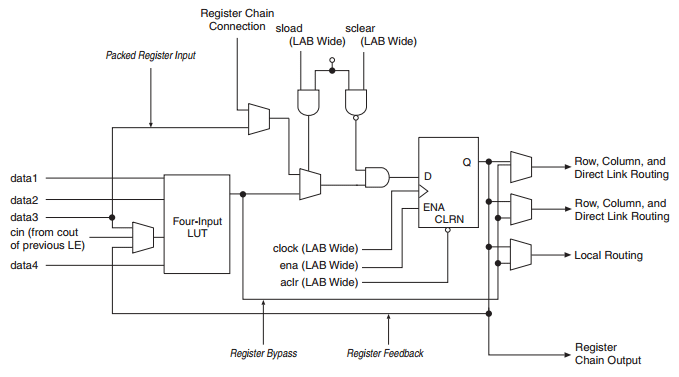
\includegraphics[width=2.5in]{LogicElement}
\caption{Cyclone III Device Family LEs in Normal Mode \cite{CycloneHandbook}}
\label{fig_LogicElement}
\end{figure}

\section{Implementation Requirements}
It was determined that an FPGA capable of at least 256 bytes of internal ROM and more than 9,000 logical elements or LE' s would be required to succefully implement the processor. As an added convenience, it was important to select a development board that would be able to handle the project inputs and outputs such as PS2 keyboard and VGA output in order to spend more time on the study and not building miscellaneous hardware.  From this research, it was determined that the Altera DE0 development board sufficiently the project needs with over 15,000 LE's, a VGA port, a PS2 port, buttons, LEDs, switches, and USB interface. Another important addition to the board is it's SecureDigital (SD) memory card slot which would be used to store the MS-DOS files.

This study has been sponsored by the Altera University Program in which they have provided an Altera DE0 development board as well as an Altera DE0-Nano development boards at no cost. This makes the projects overall required budget \$0 since the sponsorship includes the relevant packages for creating hardware on the chip.

\section{Procedure}
The Zet Processor is more than just verilog code for an Intel 8086 microprocessor, it also contains the necessary BIOS and drivers for treating the SD memory card as a mounted hard disc. The preliminary steps for installing the processor first include compiling the BIOS by running it through the OpenWatcom compiler which takes the BIOS code written in C and compiles it into x86 Assembly optimized for 16-bit instructions \cite{Watcom}. We then take the BIOS assembly and convert it into hexadecimal by means of a simple file conversion script, this is now our ROM for placing onto the FPGA. The BIOS then gets placed onto the FPGA through running the DE0\_Control\_Panel, an example program that comes with the FPGA software, that allows for files to be placed directly onto the on-board flash memory. This is important because when the processor boots, it will automatically look at address 0x00000 for instructions on where to next proceed such as how to mount the operating system and ultimately boot it. 

Since the processor runs 16-bit x86 it is necessary to choose a compatible operating system. This leaves a few options including MS-DOS 6.22, FreeDOS 1.1, and Microsoft Windows 3.0. MS-DOS was chosen due to it's small file size and easy to work with command line interface, as an added bonus since the copyright for MS-DOS has since expired it is very easy and convenient to find the source code in various places on the Internet. To load the operating system, it was necessary to load the files exactly as described from the downloaded image. The process was accomplished by running {\tt dd if=./c.img of=/dev/sdc} on a Linux computer, this instruction mounts the MS-DOS image byte-by-byte onto the SD memory card which is necessary because the BIOS looks at a specific memory location to start the operating system.

In order to begin the process of loading the processor hardware onto the FPGA, it is first important to read the documentation and manuals for the Altera DE0 Development Board and accompanying Quartus II software manual. 

The process for loading verilog onto the device is fairly straightforward, that is to compile the verilog code and debug any miscellaneous warnings and compilation errors and then to utilize the on-board programmer to load the code onto the device. When loading the code it is important to take note of the different ways in which the code can be loaded. If the code is loaded through the Joint Tag Action Group (JTAG) interface, it is important to note that this only temporarily loads the hardware and all progress will be lost after powering down the device. This feature is due to the fact that JTAG is made for testing and only loads values directly into the flip-flops and accompanying hardware but does not save this setup data to the flash memory. Since this method only sets the hardware, it can load the hardware almost instantaneously. The other method for loading hardware is known as Active Serial programming (AS), this method requires that the FPGA device is placed into programming mode which can be done by flipping a switch placed on the development board. AS places the FPGA configuration data into FLASH memory which is read into the device at power up. 

\section{Results}

\section{Problems Faced \& Troubleshooting}

\section{Conclusion \& Trends in Industry}


% use section* for acknowledgment
\section*{Acknowledgment}
The author would like to thank the Altera University Program \cite{UniProgram} for providing development boards and necessary software for work on this research.

\appendix
\label{App:AppendixA}
\subsection{Full specifications for Altera DE0 development board:}
\begin{itemize}
\item FPGA
	\begin{itemize}
 	\item Cyclone III 3C16 FPGA
	\item 15,408 LEs
	\item 56 M9K Embedded Memory Blocks
	\item 504K total RAM bits
	\item 56 embedded multipliers
	\item 4 PLLs
	\item 346 user I/O pins
	\item FineLine BGA 484-pin package
	\end{itemize}
\item Memory
	\begin{itemize}
	\item SDRAM
		\begin{itemize}
		\item One 8-Mbyte Single Data Rate Synchronous Dynamic RAM memory chip
		\end{itemize}
	\item Flash memory
		\begin{itemize}
		\item 4-Mbyte NOR Flash memory
		\item Support Byte (8-bits)/Word (16-bits) mode
		\end{itemize}
	\item SD card socket
		\begin{itemize}
		\item Provides both SPI and SD 1-bit mode SD Card access
		\end{itemize}
	\end{itemize}
\item Interface
	\begin{itemize}
	\item Built-in USB Blaster circuit
		\begin{itemize}
	 	\item On-board USB Blaster for programming
		\item Using the Altera EPM240 CPLD
		\end{itemize}
	\item Altera Serial Configuration device
		\begin{itemize}
		\item Altera EPCS4 serial EEPROM chip
		\end{itemize}
	\item Pushbutton switches
		\begin{itemize}
		\item 3 pushbutton switches
		\end{itemize}
	\item Slide switches
		\begin{itemize}
		\item 10 Slide switches
		\end{itemize}
	\item General User Interfaces
		\begin{itemize}
		\item 10 Green color LEDs
		\item 4 seven-segment displays
		\end{itemize}
	\item Clock inputs
		\begin{itemize}
		\item 50-MHz oscillator
		\end{itemize}
	\item VGA output
		\begin{itemize}
		\item Uses a 4-bit resistor-network DAC
		\item With 15-pin high-density D-sub connector
		\item Supports up to 1280x1024 at 60-Hz refresh rate
		\end{itemize}
	\item Serial ports
		\begin{itemize}
		\item One RS-232 port (Without DB-9 serial connector)
		\item One PS/2 port
		\end{itemize}
	\item Two 40-pin expansion headers
		\begin{itemize}
		\item 72 Cyclone III I/O pins, as well as 8 power and ground lines, are brought out to two 40-pin expansion connectors
		\item40-pin header is designed to accept a standard 40-pin ribbon cable used for IDE hard drives 
		\end{itemize}
	\end{itemize}
\end{itemize}

\label{App:AppendixB}
\subsection{Available x86 Instructions on the Zet Processor \cite{ZetStatus}:}

{\noindent\bf Data transfer instructions} \\
mov, push/pop, in/out, lahf/sahf, lds/lea/les, pushf/popf, xchg, xlat

{\noindent\bf Arithmetic instructions} \\
aaa/aas, aam, aad, daa/das, cbw/cwd, inc, dec, add/adc, sub/sbb, mul/imul, div/idiv, neg, cmp

{\noindent\bf Bitwise handling instructions} \\
and/or, not, rcl, rcr, rol, ror, sal/shl, sar, shr, test, xor

{\noindent\bf Control transfer instructions} \\
call, ja/jnbe, jae/jnb/jnc, jb/jnae/jc, jbe/jna, jcxz, je/jz, jg/jnle, jge/jnl, jl/jnge, jle/jng, jne/jnz, jno, jnp/jpo, jns, jmp, jo, jp/jpe, js, loop, loope/loopz, loopne/loopnz, ret

{\noindent\bf String handling instructions}\\
cmpsb/cmpsw, lodsb/lodswm, movsb/movsw, rep (pref), repe/repz (pref), repne/repnz (pref), scasb/scasw, stosb/stosw

{\noindent\bf Interrupt instructions} \\
int, into, iret

{\noindent\bf Microprocessor control instructions} \\
clc, cld, cli, cmc, hlt, nop, stc, std

% trigger a \newpage just before the given reference
% number - used to balance the columns on the last page
% adjust value as needed - may need to be readjusted if
% the document is modified later
%\IEEEtriggeratref{8}
% The "triggered" command can be changed if desired:
%\IEEEtriggercmd{\enlargethispage{-5in}}

% references section

\bibliographystyle{IEEEtran}
\bibliography{ieee_paper_contest}


\end{document}


